\documentclass[tikz,border=10pt]{standalone}
\usepackage{amsmath,amssymb}
\usepackage{tikz}
\usetikzlibrary{arrows,automata,backgrounds,calendar,chains,decorations,decorations.pathreplacing,decorations.text,fit,matrix,mindmap,patterns,petri,plotmarks,positioning,shadows,shapes,shapes.callouts,shapes.geometric,shapes.misc,spy,trees,calc,intersections,tikzmark,arrows.meta}
\usepackage{xcolor}
\usepackage{pgfplots}
\pgfplotsset{compat=1.16}

% Common math macros from the book
\def\x{\mathbf{x}}
\def\y{\mathbf{y}}
\def\z{\mathbf{z}}
\def\A{\mathbf{A}}
\def\b{\mathbf{b}}
\def\c{\mathbf{c}}
\def\w{\mathbf{w}}
\def\v{\mathbf{v}}
\def\u{\mathbf{u}}
\def\e{\mathbf{e}}
\def\zero{\mathbf{0}}
\def\R{\mathbb{R}}
\def\N{\mathbb{N}}
\def\Z{\mathbb{Z}}
\def\Q{\mathbb{Q}}
\def\st{\text{s.t.}}
\def\vect#1{\mathbf{#1}}
\def\xLP{x^{\mathrm{LP}}}
\def\zLP{z^{\mathrm{LP}}}
\def\xIP{x^{\mathrm{IP}}}

% Common node styles from the book
\tikzset{
    main/.style={circle, draw, fill=gray!20, minimum size=1cm, font=\normalsize},
    dot/.style={circle,fill=blue,minimum size=3pt,inner sep=0pt, outer sep=-1pt},
    vertex/.style={circle,fill=black!25,minimum size=20pt,inner sep=0pt},
    edge/.style={draw,-,thick},
    directed edge/.style={draw,->,>=latex,thick},
}

% Additional macros for 3D/coordinate systems
\newcommand{\xhat}{\hat{\x}}
\newcommand{\yhat}{\hat{\y}}
\newcommand{\zhat}{\hat{\z}}
\newcommand{\ihat}{\hat{\imath}}
\newcommand{\jhat}{\hat{\jmath}}
\newcommand{\khat}{\hat{k}}

\begin{document}
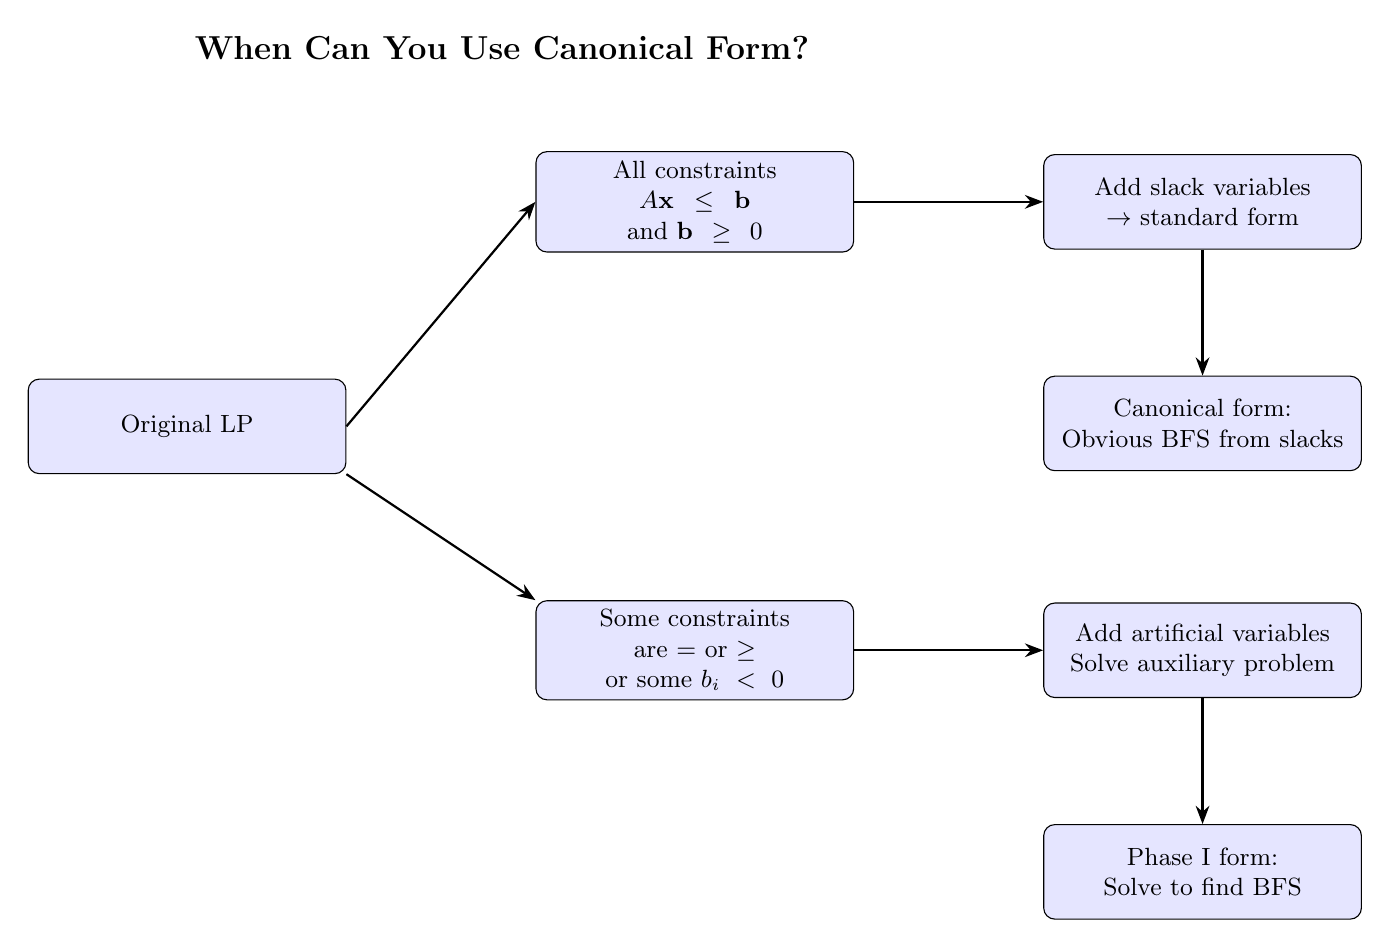
\begin{tikzpicture}[
  node distance=1.6cm and 2.4cm,
  every node/.style={font=\small},
  box/.style={draw, rounded corners, fill=blue!10, text width=3.8cm, align=center, minimum height=1.2cm},
  arrow/.style={-{Stealth}, thick}
]

% Nodes
\node[box] (start) {Original LP};
\node[box, above right=of start] (case1) {All constraints\\ $A\mathbf{x} \leq \mathbf{b}$\\ and $\mathbf{b} \geq 0$};
\node[box, right=of case1] (stdform) {Add slack variables\\ $\rightarrow$ standard form};
\node[box, below=of stdform] (canonform) {Canonical form:\\ Obvious BFS from slacks};

\node[box, below right=of start] (case2) {Some constraints\\ are $=$ or $\geq$\\ or some $b_i < 0$};
\node[box, right=of case2] (phase1) {Add artificial variables\\ Solve auxiliary problem};
\node[box, below=of phase1] (phase1form) {Phase I form:\\ Solve to find BFS};

% Arrows
\draw[arrow] (start.east) -- (case1.west);
\draw[arrow] (case1.east) -- (stdform.west);
\draw[arrow] (stdform.south) -- (canonform.north);

\draw[arrow] (start.south east) -- (case2.north west);
\draw[arrow] (case2.east) -- (phase1.west);
\draw[arrow] (phase1.south) -- (phase1form.north);

% Title
\node[align=center, font=\bfseries\large] at (4,4.8) {When Can You Use Canonical Form?};
\end{tikzpicture}
\end{document}
